\newpage
\chapter{Analýza}
\label{ch:Analýza}
V tejto časti sa venujeme dôkladnej analýze podkladov. Jednotlivé časti sú popísané v rozsahu relevantnom pre túto prácu. Analýza je štrukturovaná na nasledovné časti:

\begin{my_itemize}
	\item {Zvolená problémová oblasť}
	\item {Dáta sprístupnené pre prácu}
	\item {Dostupné metódy}
	\item {Výskum v danej oblasti}
\end{my_itemize}

\section{Zvolená problémová oblasť}
\label{problemova_oblast}

\subsection{Úbytok zákazníkov}
\label{ubytok_zakaznikov}

V tejto práci sa zameriavame na predikciu úbytku zákazníkov(churn rate) pri predplatiteľských službách. V súčasnej dobe sa do popredia biznis prístupov stále viac dostávajú prístupy riadenia vzťahov zo zákazníkmi(customer relationship management). Ukazuje sa totiž, že na trhu s dostatočným pokrytím poskytovateľov cieľovej služby je niekoľkonásobne drahšie získať si nového ako udržať si existujúceho zákazníka. Tento prístup však vyžaduje rozsiahlu znalosť dostupnej zákazníckej základne, ktorou poskytovateľ disponuje. \newline
Predikcia úbytku zákazníkov sa venuje spracovaniu dostupných informácií o zákaznickej aktivite, službách ktoré využívajú a vývoja ich správania v čase. Výsledkom takejto analýzy je štatistika poskytujúca informácie o jednotlivých zákazníkoch a ich šanci na presun k inému poskytovateľovi. Z týchto dát je následne odvoditeľné, aké percento zákazníkov odíde ku konkurencii a aký to bude mať dopad na finančné príjmy od ktorých je poskytovateľ závislý. 

\subsection{Moderovanie úbytku zákazníkov}

Vo vzťahu k úbytku zákazníkov definuje CRM dva základné prístupy, ktorými je možné moderovať úbytok. 


\subsubsection{Reaktívny prístup}
\label{reaktivny_pristup}

Motivácia zákazníka pre zotrvanie s pôvodnym poskytovateľom služby nastáva, až keď sa zákazník explicitne rozhodne pre prechod ku konkurenčnému poskytovateľovi. V tomto okamihu začína poskytovateľ na svojho zákazníka apelova výhodnými ponukami, zľavami alebo inými spôsobmi motivácie pre zotrvanie u poskytovateľa. Takýto prístup sa ukazuje ako ľahko zneužiteľný ostatnými zákazníkmi, ktorí by inak nemali motiváciu pre prechod ku konkurencii. Predikcia úbytku zákazníkov v tomto prístupe nemá nijakú významnú úlohu.

\subsubsection{Proaktívny prístup}
\label{proaktivny_pristup}

Pri úspešnej predikcií záujmu zákazníka o prechod ku konkurenčnému poskytovateľovi je možné efektívne jeho zámer smerovať pozitívnou motiváciou. Tentoo prístup však predpokladá vysokú úspešnosť predikčných metód. Pri nesprávnej identifikácii zákazníckeho správania je totiž možné nielen nezabrániť zákazníkom v presune ku konkurenčnému modelu, ale aj investícii finančných prostriedkov do skupiny zákazníkov, ktorá by naďalej generovala zisk aj bez významnejšej motivácie, resp. nevrátila by rozdielom v úbytku motivačné náklady, ktoré na ňu daný poskytovateľ vynaložil.


\section{Časť}
\label{sec:Časť}
V tejto časti sa venujeme 
\begin{figure}[H]
\begin{center}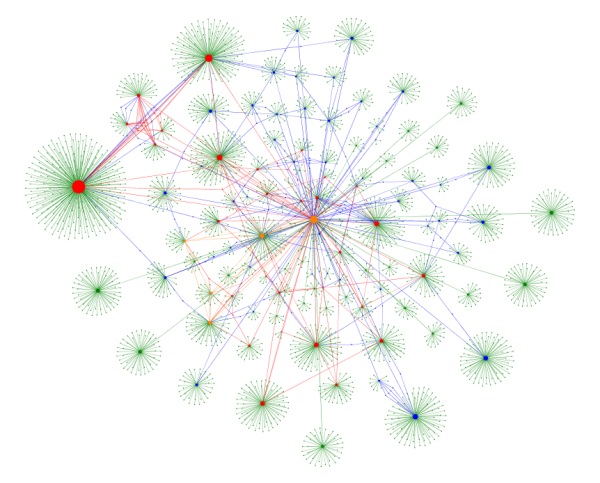
\includegraphics[scale=0.48]{figure}\end{center}
\caption[Name figure]{Name figure}\label{fig:figure}
\end{figure}

%\subsection{Enumeration}
\subsection{Číslovaný zoznam}
\begin{my_enumerate}
	\item {cieľ 1}
	\begin{my_enumerate}
		\item {cieľ 1.a}
		\item {cieľ 1.b}
	\end{my_enumerate}
	\item {cieľ 2}
	\item {cieľ 3}
\end{my_enumerate}

%\subsection{Citation}
\subsection{Citácia}
Lorem ipsum dolor sit amet, consectetuer adipiscing elit, sed diam nonummy nibh euismod tincidunt ut laoreet dolore magna aliquam erat volutpat~\cite{1}.

%\subsection{Labels \& References}
\subsection{Návestia \& Referencie}
Viď. sekcia~\ref{sec:Príklady}.\\
Viď. ukážka~\ref{fig:ukážka}.\\
Viď. číslovanie~\ref{lst:metrics_LOC}.\\
Viď. tabuľka~\ref{tab:tabuľka1}.

%\subsection{Examples}
\subsection{Príklady}
\label{sec:Príklady}

\begin{lstlisting}[ language=html, caption={Príklad 1}, label={lst:metrics_LOC},
	keywordstyle=\color{blue}\bfseries,
	ndkeywordstyle=\color{black}\bfseries,
	commentstyle=\color{red}\ttfamily,
	stringstyle=\color{green}\ttfamily,
	identifierstyle=\color{gray},
	backgroundcolor=\color{white}, 
	frame=single, 
	frameround=ffff,
	captionpos=b,
	basicstyle=\scriptsize
	]
<table class="metric_index">
	<tr>
		<th>Lines of code</th>
		<th>Value</th>
	</tr>
	<% if (filenum and modulenum) then %>
		<tr>
			<td class="name">Number of files</td>
			<td class="value"><%=filenum%></td>
		</tr>
		<tr>
			<td class="name">Number of modules</td>
			<td class="value"><%=modulenum%></td>
		</tr>
		<tr>
	<% end %>
	<tr>
		<td class="name">Lines Total</td>
		<td class="value"><%=LOC.lines%></td>
	</tr>
	<!--
							skryty zdrojovy kod
		podobne zobrazenie ostatnych metrik riadkov
	-->
</table>
\end{lstlisting}

\begin{lstlisting}[language=lua, caption={Názov}, label=metrics.pipe]
local parser  = require 'leg.parser'
local rules = require 'metrics.rules'
-- << skryty zdrojovy kod >> --
local capture_table = {}
grammar.pipe(LOC_capt.captures, AST_capt.captures)
grammar.pipe(block_capt.captures, LOC_capt.captures)
-- << viacero rovnakych volani s tabulkami captures inych modulov >> --
grammar.pipe(capture_table, cyclo_capt.captures)
local lua = lpeg.P(grammar.apply(parser.rules, rules.rules, capture_table))
local patt = lua / function(...) 
	return {...} 
end
local result = patt:match(code)[1]
\end{lstlisting}

\begin{lstlisting}[language=C++, tabsize=2, caption={Manager}]
int a;
\end{lstlisting}



\begin{table}[ht]
    \centering
    \begin{tabular}{ | l | l | }
    \hline
    Number of males & 51 \\ \hline
    Number of woman & 57 \\ \hline
    Gender not given & 27 \\ \hline
    Average age & 21,83 \\ \hline
    \end{tabular}
    \caption{Information about users}
    \label{tab:table1}
\end{table}
